\let\negmedspace\undefined
\let\negthickspace\undefined
\documentclass[journal]{IEEEtran}
\usepackage[a5paper, margin=10mm, onecolumn]{geometry}
\usepackage{tfrupee}

\setlength{\headheight}{1cm}
\setlength{\headsep}{0mm}

\usepackage{gvv-book}
\usepackage{gvv}
\usepackage{cite}
\usepackage{amsmath,amssymb,amsfonts,amsthm}
\usepackage{algorithmic}
\usepackage{graphicx}
\usepackage{textcomp}
\usepackage{xcolor}
\usepackage{txfonts}
\usepackage{listings}
\usepackage{enumitem}
\usepackage{mathtools}
\usepackage{gensymb}
\usepackage{comment}
\usepackage[breaklinks=true]{hyperref}
\usepackage{tkz-euclide}
\usepackage{listings}
\def\inputGnumericTable{}
\usepackage[latin1]{inputenc}
\usepackage{color}
\usepackage{array}
\usepackage{longtable}
\usepackage{calc}
\usepackage{multirow}
\usepackage{hhline}
\usepackage{ifthen}
\usepackage{lscape}

\begin{document}

\bibliographystyle{IEEEtran}
\vspace{3cm}

\title{4.13.8}
\author{EE25BTECH11003 - Adharvan Kshathriya Bommagani}
{\newpage\maketitle}

\renewcommand{\thefigure}{\theenumi}
\renewcommand{\thetable}{\theenumi}
\setlength{\intextsep}{10pt}

\textbf{Question}:\\
The orthocentre of the triangle formed by the lines $x + y = 1$, $2x + 3y = 6$ and $4x - y + 4 = 0$ lies in the quadrant number \rule{1cm}{0.15mm}.

\bigskip

\textbf{Solution}:\\

The three lines, written in the vector normal form $\mathbf{n}^\top \mathbf{x} = c$, are:
\begin{align}
     L_1: \myvec{1 \\ 1}^\top \myvec{x \\ y} = 1\\
     L_2: \myvec{2 \\ 3}^\top \myvec{x \\ y} = 6\\
     L_3: \myvec{4 \\ -1}^\top \myvec{x \\ y} = -4
     \end{align}
The vertices $\vec{A}$, $\vec{B}$, $\vec{C}$ are the intersection points of these lines. We solve for them using gaussian elimination(row reduction).

Vertex $\vec{A}$: Intersection of $L_1$ and $L_2$
The system is: $x+y=1$ and $2x+3y=6$.
Augmented matrix:

\begin{align}
   \myaugvec{2}{
1 & 1 & 1 \\
2 & 3 & 6
} 
\end{align}


Apply the row operation $R_2 \to R_2 - 2R_1$:
\begin{align}
\myaugvec{2}{
1 & 1 & 1 \\
0 & 1 & 4
}
\end{align}
From the second row, $y=4$. Substituting into the first row ($x+y=1$), we get
\begin{align}
    x+4=1 \implies x=-3.
\end{align}


\begin{align}
    \vec{A}=\myvec{-3 \\ 4}
\end{align}

Vertex $\vec{B}$: Intersection of $L_2$ and $L_3$
The system is: $2x+3y=6$ and $4x-y=-4$.
Augmented matrix:
\begin{align}
\myaugvec{2}{
2 & 3 & 6 \\
4 & -1 & -4
}
\end{align}
Apply the row operation $R_2 \to R_2 - 2R_1$:
\begin{align}
\myaugvec{2}{
2 & 3 & 6 \\
0 & -7 & -16
}
\end{align}
From the second row, 
\begin{align}
-7y=-16 \implies y=\frac{16}{7}. 
\end{align}

Substituting into the first row ($2x+3y=6$), we get
\begin{align}
2x+3(\frac{16}{7})=6 \implies 2x = 6 - \frac{48}{7} = -\frac{6}{7} \implies x=-\frac{3}{7}.
\end{align}
\begin{align}
    \vec{B}=\myvec{-\frac{3}{7} \\ \frac{16}{7}}
\end{align}

Vertex $\vec{C}$ : Intersection of $L_1$ and $L_3$ 
The system is: $x+y=1$ and $4x-y=-4$.
Augmented matrix:

\begin{align}
\myaugvec{2}{
1 & 1 & 1 \\
4 & -1 & -4
}
\end{align}

Apply the row operation $R_2 \to R_2 - 4R_1$:
\begin{align}
\myaugvec{2}{
1 & 1 & 1 \\
0 & -5 & -8
}
\end{align}
From the second row,
\begin{align}
-5y=-8 \implies y=\frac{8}{5}
\end{align}
Substituting into the first row ($x+y=1$), we get,
\begin{align}
    x+\frac{8}{5}=1 \implies x = 1 - \frac{8}{5} = -\frac{3}{5}
\end{align}
\begin{align}
    \vec{C}=\myvec{-\frac{3}{5} \\ \frac{8}{5}}
\end{align}


\textbf{Altitude from Vertex $\vec{A}$ (AD)}:\\
This altitude passes through $\vec{A}$=\myvec{-3 \\ 4} and is perpendicular to line $L_3$.\\
A normal vector for the altitude is therefore,
\begin{align}
\myvec{1 \\ 4}. 
\end{align}
The equation is
\begin{align}
     x+4y=k.
\end{align}
Since it passes through $\vec{A}$=\myvec{-3 \\ 4}: 
\begin{align}
(-3)+4(4)=k \implies k=13.
\end{align}
\textbf{Equation of Altitude AD}: 
\begin{align}
\myvec{1 \\ 4}^\top \myvec{x \\ y} = 13.
\end{align}
\textbf{Altitude from Vertex $\vec{C}$ (CE)}:\\
This altitude passes through $\vec{C}$=\myvec{-\frac{3}{5} \\ \frac{8}{5}} and is perpendicular to line $L_2$. A normal vector for the altitude is therefore, 
\begin{align}
\myvec{3 \\ -2}
\end{align}
The equation is
\begin{align}
3x-2y=k
\end{align}
Since it passes through $\vec{C}$=\myvec{-\frac{3}{5} \\ \frac{8}{5}}:
\begin{align}
3(-\frac{3}{5})-2(\frac{8}{5})=k \implies k = -\frac{9}{5}-\frac{16}{5} = -5
\end{align}
\textbf{Equation of Altitude CE}: 
\begin{align}
\myvec{3 \\ -2}^\top \myvec{x \\ y} = -5
\end{align}

We solve the system for the two altitudes: $x+4y=13$ and $3x-2y=-5$.
Augmented matrix:
\begin{align}
\myaugvec{2}{
1 & 4 & 13 \\
3 & -2 & -5
}
\end{align}
Apply the row operation $R_2 \to R_2 - 3R_1$:
\begin{align}
\myaugvec{2}{
1 & 4 & 13 \\
0 & -14 & -44
}
\end{align}
From the second row, 
\begin{align}
-14y=-44 \implies y=\frac{44}{14}=\frac{22}{7}
\end{align}
Substituting into the first row ($x+4y=13$): 
\begin{align}
x+4(\tfrac{22}{7})=13 \implies x = 13-\frac{88}{7} = \frac{91-88}{7}=\frac{3}{7}
\end{align}
The orthocentre is 
\begin{align}
\vec{H} = \myvec{\frac{3}{7}, \frac{22}{7}}
\end{align}

The coordinates of the orthocentre are $(\frac{3}{7}, \frac{22}{7})$.
Since both the x-coordinate and y-coordinate are positive, the orthocentre lies in the first quadrant.\\

\textbf{Plot of the Lines and Orthocentre:}
\begin{figure}[H]
    \centering
    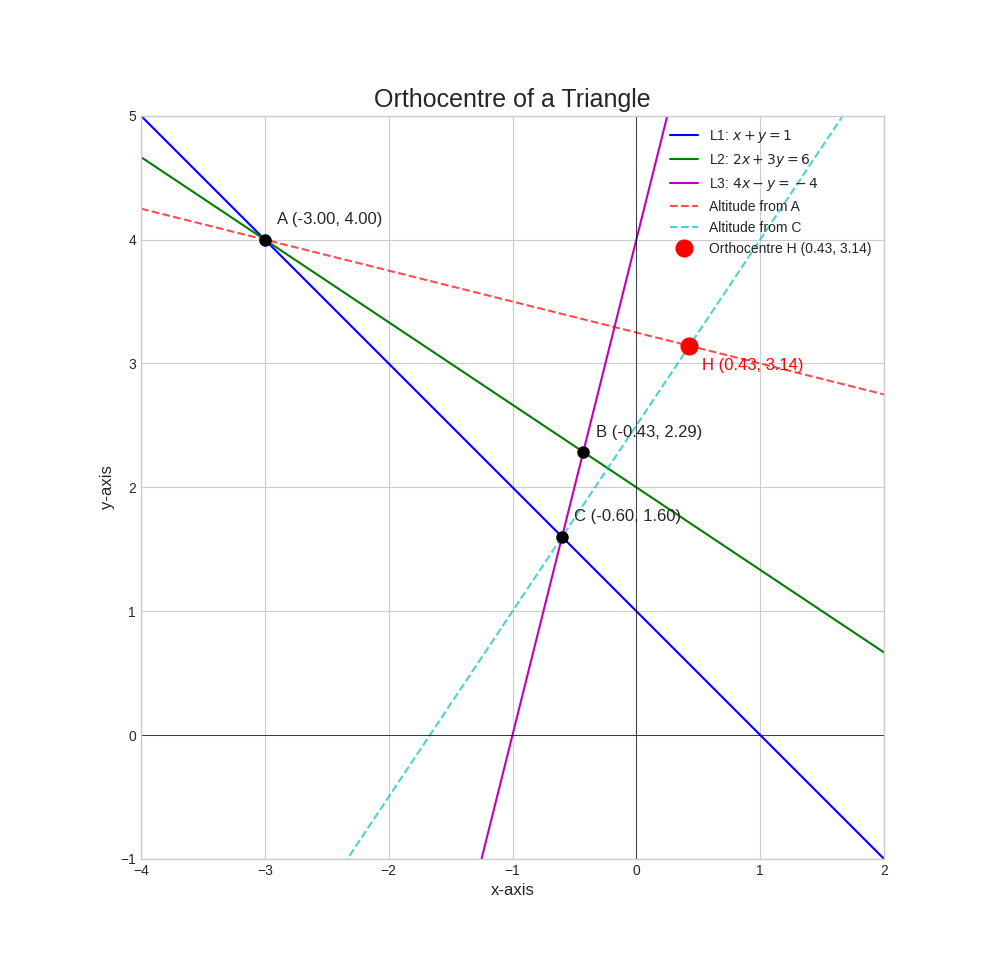
\includegraphics[width=0.9\columnwidth]{figs/fig1.png}
    \caption{Figure for 4.13.8}
    \label{}
\end{figure}

\end{document}